\documentclass[a4paper]{scrartcl}
\usepackage[round,authoryear]{natbib}
\usepackage{graphicx}
\usepackage{color}
\usepackage{lineno}
\usepackage{multirow}
\usepackage{amsmath}
\usepackage{epstopdf}
\usepackage{hyperref}
\hypersetup{
    colorlinks=true,       % false: boxed links; true: colored links
    linkcolor=red,          % color of internal links (change box color with linkbordercolor)
    citecolor=darkgreen,        % color of links to bibliography
    filecolor=magenta,      % color of file links
    urlcolor= black           % color of external links
}
\usepackage{color}
	 \definecolor{darkred}{rgb}{0.75,0,0}
	 \definecolor{darkgreen}{rgb}{0,0.5,0}
	 \definecolor{darkblue}{rgb}{0,0,0.75}

\newcommand{\cha}[1]{\textcolor{blue}{#1}}

\usepackage{setspace}

\newcommand{\fig}[1]{Fig.~\ref{fig:#1}}
\newcommand{\Fig}[1]{Figure~\ref{fig:#1}}
\newcommand{\figs}[2]{Figures~\ref{fig:#1},~\ref{fig:#2}}
\newcommand{\eq}[1]{Eq.~\ref{eq:#1}}
\newcommand{\sect}[1]{Section~\ref{sect:#1}}
\newcommand{\app}[1]{Appendix~\ref{app:#1}}
\newcommand{\esm}[0]{\textcolor{red}{ESM}}

\begin{document}
\sffamily
\title{
On multiple infections by parasites with complex life cycles
}   
%\author{Chaitanya S.~Gokhale$^{\dag \star}$, Arne Traulsen$^{\dag}$ and Gerrit Joop$^{\ddag}$\\
%\small{$^\dag$Department of Evolutionary Theory,}\\
%\small{Max Planck Institute for Evolutionary Biology,}\\
%\small{August-Thienemann-Stra{\ss}e 2, 24306 Pl\"{o}n, Germany}\\
%\small{$^\ddag$Institut f\"ur Insektenbiotechnologie, University of Giessen,}\\
%\small{Evolutionary Ecology and Genetics, University of Kiel, Germany}\\
%\small{$^\star$gokhale@evolbio.mpg.de}
%}

\date{}
\maketitle

\onehalfspacing

\linenumbers

\begin{abstract}
{
\sffamily
Host manipulation is a common strategy of parasites of different complexity. 
It directly affects predator-prey dynamics in trophically transmitted parasites, where parasite transmission requires predation. Theoretical studies suggest that manipulation that enhances predation often results in a heavy burden on the prey population. 
Consequently, the system is often destabilised, making parasites prone to extinction. 
Host manipulation, however, can also suppress predation.
Such suppression is possible if multiple parasites coinfect a host with conflicting interests in manipulation. 
The interests could be misaligned for various reasons, such as limited carrying capacity or parasitoid developmental stage.
Multiple infections are a norm in parasite ecology but are often neglected in the theoretical assessment of host-parasite dynamics.
We tease apart the effect of host manipulation of coinfected parasites and manipulation interests via a mathematical model of a trophically transmitted parasite with a complex life cycle.
The life cycle comprises a free-living state, an intermediate and a definitive host. 
With coinfection, we show that host manipulation that enhances predation need not permanently destabilise the predator-prey system. 
However, sabotage in manipulation can induce bistability such that a slight disturbance in the system drives the parasite population to extinction. 
Intriguingly, cooperation in host manipulation and synergism in reproduction might not ensure system stability. 
In some cases, depressed reproduction in co-infecting parasites may prevent the dynamical system from bistability.
Our study highlights the necessity and means of incorporating the reality of multiple parasites and their multi-trophic life cycles in a single system in studying parasite ecology.
}
\end{abstract}

\sffamily

\section*{Introduction}

% The journal does not have numbered sections in the main portion of
% articles. Please refrain from using section references (à la
% section~\ref{section:CountingOwlEggs}), and refer to sections by name
% (e.g. section ``Counting Owl Eggs'').

Parasites infect life on earth ubiquitously, and many of these parasites have complex life cycles \citep{zimmer:book:2001}. 
While a complex lifecycle can be defined as abrupt ontogenic changes in morphology and ecology \citep{Benesh:2016dj}, a complex parasitic lifecycle typically involves numerous hosts that a parasite needs to traverse to complete its life cycle. 
This complex lifecycle results in the evolution of various strategies that enable the success of parasite transmission from one host to another. 
One famous strategy that inspires many science fiction movies and novels is host manipulation, where a parasite can alter the morphology and/or behaviour of its  host to enhance its transmission to the next host \citep{Hughes2012}. 
Host manipulation has been shown in many host-parasite systems, from parasites with simple life-cycle to those with complex life-cycle that involves more than one host \citep{Hughes2012,molyneux_jefferies1986}. 
For instance, sand flies infected by \textit{Leishmania} parasites bite more and take more time for a blood meal from mammals (the definitive host of \textit{Leishmania}) compared to their uninfected counterparts \citep{Rogers2007}. 
Copepods infected by cestode parasites are more active and accessible to sticklebacks (the definitive hosts of the cestodes) compared to uninfected copepods \citep{Wedekind1996}.

Theoretical studies have long attempted to understand the ecological and evolutionary consequences of host manipulation. 
\cite{Roosien2013} and \cite{Hosack2008} showed that manipulative parasites could increase the disease prevalence in an epidemic. \cite{Gandon2018} studied the evolution of the manipulative ability of infectious disease parasites, showing different evolutionary outcomes depending on whether the pathogen can control its vector or host.
\cite{Hadeler1989, Fenton2006} and \cite{Rogawa2018} showed that host manipulation could stabilise or destabilise the predator-prey dynamics depending on how manipulation affects the predation response function and the assumption on the fertility of the definitive infected host. 
\cite{Seppl2008} showed that host manipulation could evolve even when it increases the risk of the intermediate host being eaten by a non-host predator, given that the initial predation risk is sufficiently low. 
These models, however, lack a crucial aspect of parasite dynamics, multiple infections \citep{kalbe:JFB:2002} 

Typical studies do not consider multiple infections, a phenomenon that is the norm rather than an exception in parasitism. 
Multiple infections result in the coinfection of more than one parasite inside a host, which may alter the manipulative outcomes (figure \ref{fig:empirical}). 
An alignment of interest between coinfecting parasites may enhance manipulation, while a conflict of interest may reduce the manipulative effect. 
Indeed, \cite{Hafer:2015gl} showed that copepods infected by two cestode parasites reduce the activity of copepods when both parasites are at the same noninfectious stage, i.e. both parasites are not ready to transmit. 
Thus the reduction in mobility is suggested to reduce the predation rate by the definitive hosts. 
When two infectious parasites infect the copepods, the copepods' activity increases, and so does the predation risk for the copepod. 
However, when the copepods are infected by one infectious and one noninfectious parasite, their interests clash, and one parasite wins over the other. 

\begin{figure}[ht!]
\centering
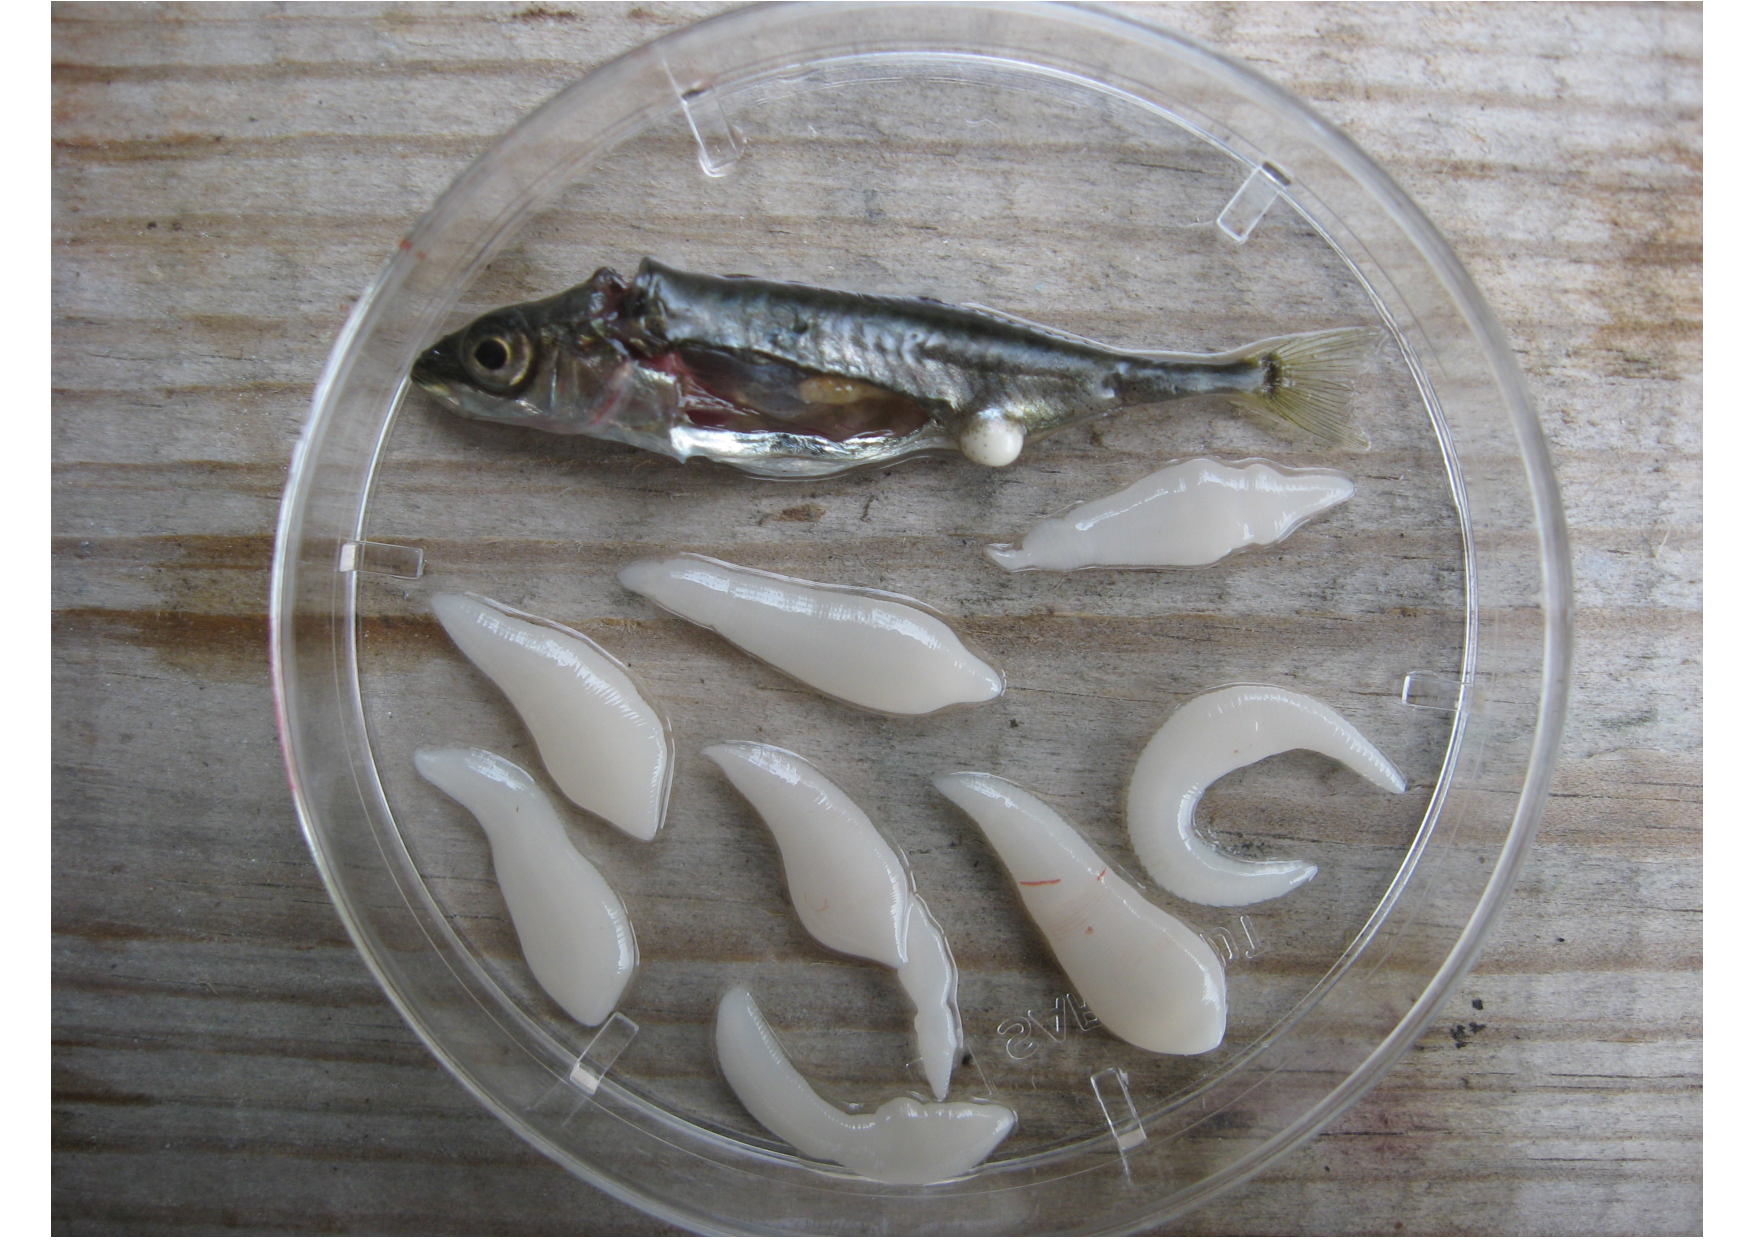
\includegraphics[width=0.75\columnwidth]{Figures/Sept_10_ 101.pdf}
\caption{\textbf{Who is in control?.}
Schistocephalus eggs, which overwinter at the bottom of bodies of water, hatch into microscopically small swimming larvae. 
These larvae are eaten by copepods (also known as Cyclops due to its single eye), where they develop to the second larval stage. 
However, the copepod is only the first intermediate host. 
The larvae are then eaten by sticklebacks, where they reach the third larval stage and grow significantly in size and weight. 
For the parasite to successfully reach its final host, a warm-blooded animal like a bird, it manipulates its intermediate hosts. 
The timing is crucial as the chances of success are greatest if the larvae develop in the copepod for 13 to 15 days before entering the stickleback. 
The presence of multiple parasites in the same host can lead to competition and strategic decision pertaining to investment in manipulation and growth.
And indeed a stickleback can be infected by numerous tapeworms as shown above by Martin Kalbe.
}
\label{fig:empirical}
\end{figure}


Theoretical work that considers multiple infections often focuses on the evolution of virulence \citep{vanBaalen1995, Alizon2013, Alizon2008, Choisy2010, Alizon2012}. 
They show multiple infections can increase virulence \citep{vanBaalen1995, Choisy2010}.
Evolutionary branching of a less virulent and a hypervirulent parasite can occur when considering within-host dynamics \citep{ Alizon2008}, and a reduction in virulence is possible if parasites are co-transmitted \citep{Alizon2012}. 
These studies also involve host manipulation to a certain extent, as it can affect transmission rates, even though they do not explicitly consider the trait. 
Host manipulation in trophically transmitted parasites receives less attention. 
Although manipulation correlates with the transmission rate in trophically transmitted parasites and infectious diseases, there are differences. 
Host manipulation influences the predation rate in trophically transmitted parasites, predominantly affecting predator-prey dynamics. 
Theoretical studies on host manipulation in trophically transmitted parasites with multiple infections are rare \citep{Parker2003,Vickery2009}. 
Moreover, they do not consider the prey-predator dynamics, which will likely have important feedback on the evolution of host manipulation. 
A few studies considering the prey-predator dynamics do not incorporate multiple infections \citep{Rogawa2018, Iritani2018, Hadeler1989, Fenton2006}. 
More importantly, they assume that transmission from definitive hosts to intermediate hosts is due to direct contact between the two types of hosts. 
This is often not the case, as parasites are released from the definitive hosts into the environment. 
Transmission happens only when intermediate hosts have contact with this free-living parasite pool.

Our study addresses the gap in the theoretical work on host manipulation in trophically transmitted parasites.
We include multiple infections and consider the dynamics of the free-living parasite pool. 
Our compartment model helps illustrate a parasite's complex lifecycle with two hosts: an intermediate host preyed upon by a definitive host. 
Transmission from the intermediate host to the definitive host occurs when predation on infected intermediate hosts happens. 
Reproduction only happens in the definitive hosts. 
New parasites then enter the environment, where the cycle continues. 
We focus on the intermediate host manipulation, such that the parasite increases the uptake of the intermediate host by the definitive host to increase its transmission rate. 
We then analyse the effect of host manipulation on the ecological dynamics in the prey-predator-parasite system. 
In contrast to the abovementioned examples, our model consists of a single intermediate host as it already provides enough complexity to discuss between transmission and manipulation.
We found that sabotage in host manipulation almost always pushes the dynamical system toward bistability, provided the reproduction in a single infection is sufficiently small. 
The bistable nature suggests that the predator-prey parasite system is finely balanced and susceptible to extinction via ecological disturbances. 
Initially surprising, we showed that cooperation in host manipulation and enhanced reproduction in co-infecting parasites is not always beneficial and might expose the parasite population to the risk of extinction.

\section*{Model and Results}

Our model concerns the complex lifecycle of a trophically transmitted parasite that requires two hosts: an intermediate host and a definitive host. 
Reproduction only happens inside the definitive hosts, releasing new parasitic progeny in the environment. 
An intermediate host can be infected if it encounters this free-living parasite pool. 
Finally, when a definitive host consumes an infected intermediate host, the definitive host gets infected, and the parasite completes its lifecycle.

For simplicity, we assume that hosts can be infected by one (single infection) or, at most, two parasites (double infections). 
Our model is, therefore, more relevant to the macroparasitic system.
Given that infection occurs, the probability that two parasites from the parasite pool co-transmit to an intermediate host is denoted by  $p$. Thus $1-p$ is the probability that a single parasite enters an intermediate host. 
When a definitive host consumes an intermediate host infected by two parasites, there is a probability $q$ that the parasites co-transmit to the definitive host.
With probability $1-q$, only one parasite successfully transmits. 
This formulation assumes that infection always happens when hosts encounter parasites.
The dynamics of a complex lifecycle parasite that requires two hosts is described by the following system of equations, firstly for the intermediate host as,
%
\begin{align}
\frac{dI_s}{dt} &= R(I_s, I_w, I_{ww}) - d I_s - P_s(D_s, D_w, D_{ww}) I_s  - \eta  I_s \nonumber \\ 
\frac{dI_w}{dt} &=  (1 - p) \eta I_s  - (d + \alpha_w) I_w - P_w(D_s, D_w, D_{ww}, \beta_w) I_w \label{odes:ihosts} \\
\frac{dI_{ww}}{dt} &= p \eta I_s  - (d + \alpha_{ww}) I_{ww} - P_{ww}(D_s, D_w, D_{ww}, \beta_{ww}) I_{ww} \nonumber
\end{align}
%
where $R(I_s, I_w, I_{ww})$ represents the birth rate of the intermediate hosts, a function of both infected and uninfected individuals.
$P_s, \ P_w, \ P_{ww}$ are the predation functions of definitive hosts on susceptible, singly infected and doubly infected intermediate hosts. 
The predation function depends on the density of the definitive hosts and the manipulative strategies of parasites in the intermediate hosts. 
In particular, if a single parasite infects an intermediate host, the manipulation strategy is $\beta_w$. 
However, if the intermediate host is co-infected, the manipulation strategy is $\beta_{ww}$. 
In the scope of this model, we assume no specific relationship between $\beta_w$ and $\beta_{ww}$ to explore all possible ecological outcomes of the system. 
The force of infection by parasites in the environment is denoted by $\eta = \gamma W$. 
Since parasites can manipulate intermediate and definitive hosts, here, whenever we mention host manipulation, it specifically refers to the manipulation in intermediate hosts, which correlates to the predation rate.

For the definitive hosts we have,
%
\begin{align}
\frac{dD_s}{dt} &= B(D_s,  D_w,  D_{ww},  I_s, I_w, I_{ww})  - \mu D_s - (\lambda_{ww} + \lambda_w) D_s \nonumber \\    
\frac{dD_w}{dt} &= (\lambda_w + (1 - q) \lambda_{ww}) D_s - (\mu + \sigma_w) D_w - ((1 - q) \lambda_{ww} + \lambda_w) D_w  \label{odes:dhosts} \\         
\frac{dD_{ww}}{dt} &= q \lambda_{ww} D_s + ((1 - q) \lambda_{ww} + \lambda_w) D_w - (\mu + \sigma_{ww}) D_{ww} \nonumber
\end{align}
%
where $B(D_s, D_w, D_{ww}, I_s, I_w, I_{ww})$ represents the birth rate of definitive hosts.
The birth rates depend on the density of both intermediate and definitive hosts, infected or uninfected. 
The force of infection that corresponds respectively to singly infected intermediate host ($I_w$) and doubly infected intermediate hosts ($I_{ww}$) is denoted respectively by $\lambda_w = h_1 (\rho + \beta_w)  I_w$ and $\lambda_{ww} = h_2 (\rho + \beta_{ww}) I_{ww}$, where $\rho$ is the baseline predation rate and $h_1$ and $h_2$ are the probability that the parasite successfully established inside the host.
If there is no manipulation, that is, $\beta_w = \beta_{ww} = 0$, the parasite is still transmitted via the based line predation. 
The dynamics of the free-living parasites in the environment are then given by,
\begin{align}
	\frac{dW}{dt} &= f_w D_w + f_{ww} D_{ww} - \delta W - \eta I_s. \label{odes:eparasite}
\end{align}
%
Definitions of different parameters can be found in Table~\ref{table:varpardescription}.

Here, we focus on manipulation that enhances transmission from intermediate hosts to definitive hosts; we thus simplify the transmission from the parasite pool to intermediate hosts such that no sequential infection. 
This assumption is motivated given that the prey' lifecycle is often shorter than that of the predator \cha{citation}. 
A prey likely encounters the free-living parasite pool once and then dies due to predation, making sequential transmission less likely at this state.
Sequential infection can happen when parasites transmit from intermediate hosts to definitive hosts. 
Therefore, a singly infected definitive host can be further infected by another parasite if it consumes infected intermediate hosts. 
Figure (\ref{fig:schematic}) illustrates the system's dynamics.
%
\begin{figure}[ht!]
\centering
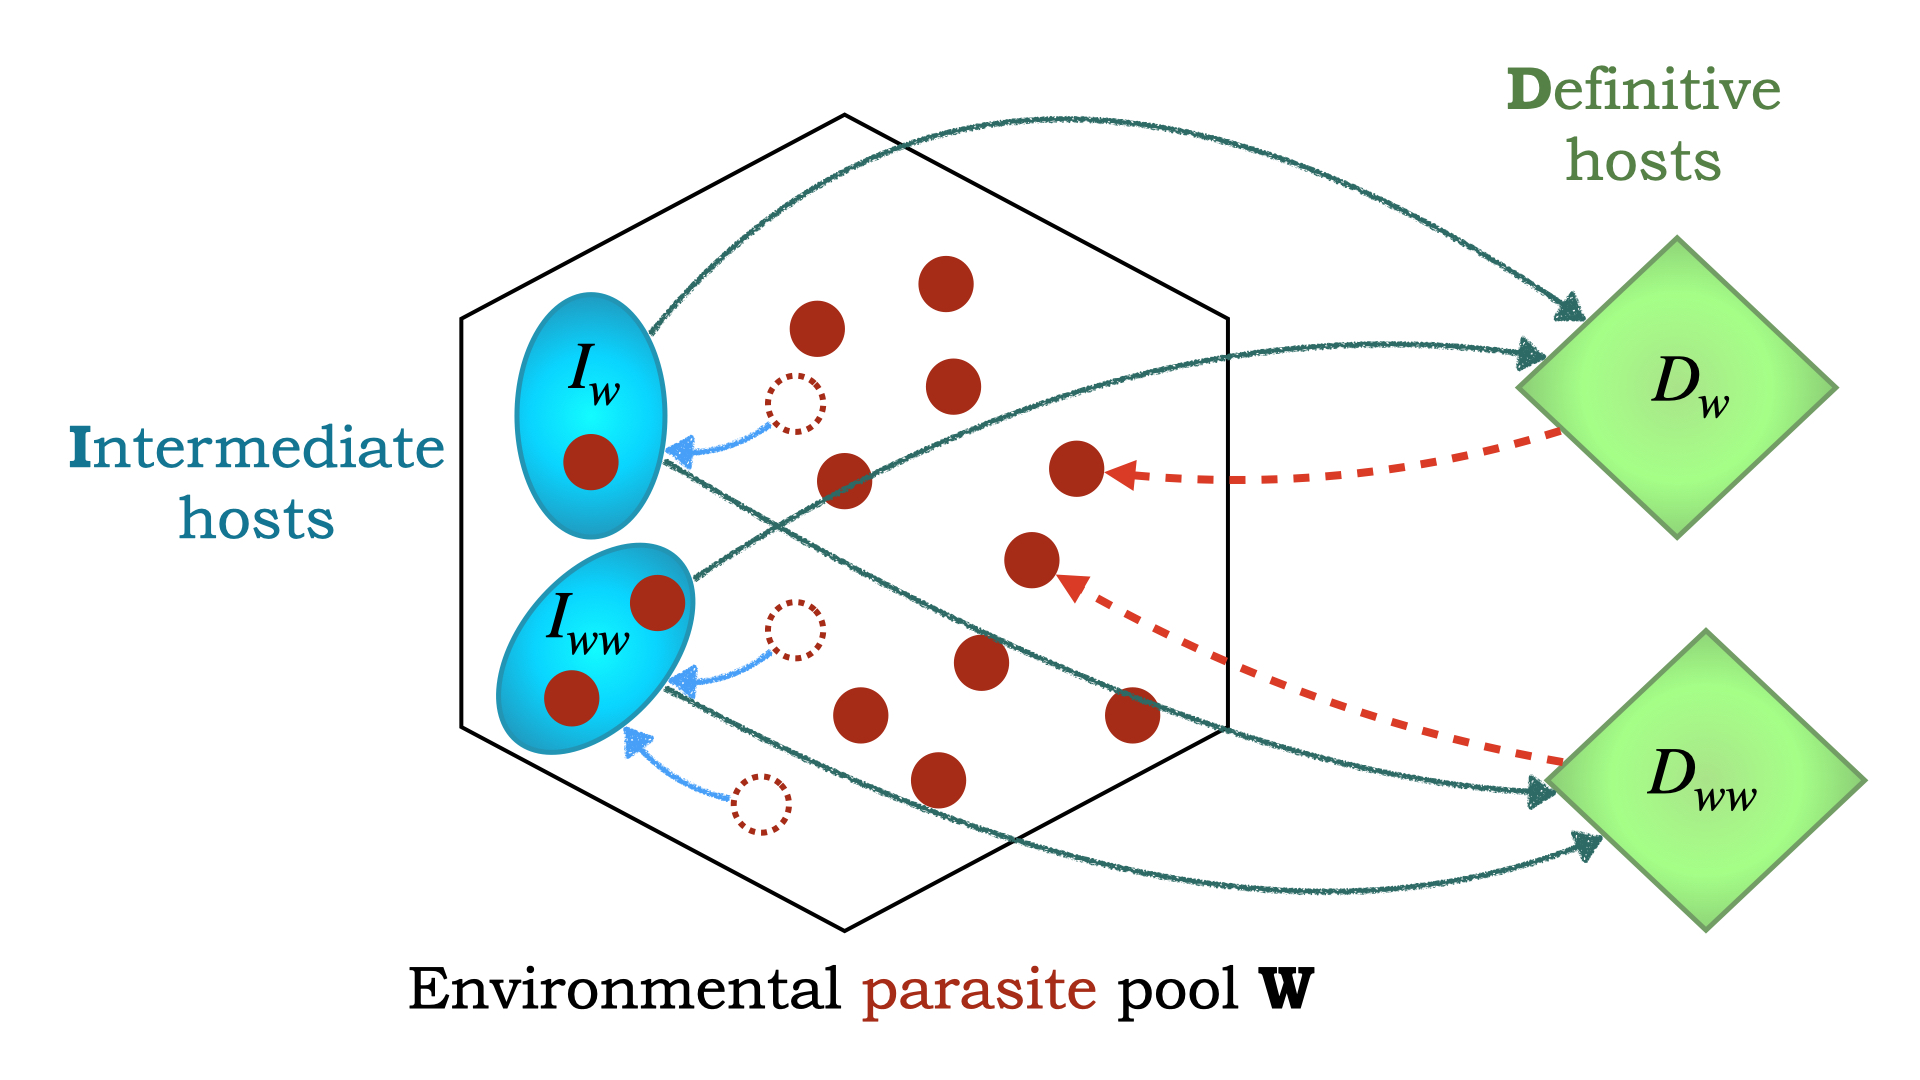
\includegraphics[width=\textwidth]{Figures/schematic.jpeg}
\caption{Schematic of the model. Blue ovales represent intermediate host compartment, 
green diamonds represent definitive host compartment, 
and the transparent hexagon represents the parasite pool compartment with red circles illustrating individual parasites.
}
\label{fig:schematic}
\end{figure}

\subsection*{Basic reproduction ratio $R_0$ of the parasites}

The basic reproduction ratio $R_0$ (or basic reproduction number as often used in epidemiology) indicates parasite fitness. 
It can be understood as the expected number of offspring a parasite produces during its lifetime when introduced to a susceptible host population. 
We calculate the basic reproduction ratio $R_0$ using the next-generation method \citep{Diekmann1990, Diekmann2009, hurford:JRSI:2010} (See SI1 for details).
%
\begin{align}
R_0 = & \overbrace{\gamma I_s^* \frac{p q h (\rho +  \beta_{ww})}{\alpha_{ww} + d + P_{ww}} \frac{D_s^*}{\mu +\sigma_{ww}} \frac{f_{ww}}{\delta +\gamma I_s^*}}^{ \texttt{Double infections}} + \nonumber \\
& \underbrace{\gamma  I_s^* \left( \frac{ (1-p) h (\rho + \beta_w)}{\alpha_w + d + P_w} + \frac{p (1-q) h (\rho + \beta_{ww})}{\alpha_{ww} + d + P_{ww}} \right) \frac{D_s^*}{\mu + \sigma_w} \frac{f_w}{\delta +\gamma  I_s^*}}_{\texttt{Single infection}}
\end{align}
%
where $I_s^*$ and $D_s^*$ are the densities of susceptible intermediate and definitive hosts at the disease-free equilibrium. 
Here, the expression of $R_0$ contains the possible reproduction routes of a parasite, which can be via double or single infections. 
The first component corresponds to the double infections route, in which the focal parasite co-transmits with another parasite into a susceptible intermediate host, then co-transmits into a susceptible definitive host and reproduces. 
Here, parasites are so rare that only co-transmission matters and the compartments with sequential infections are therefore neglected. 
The second component corresponds to the single infection route, wherein the focal parasite infects a susceptible intermediate host via single or double infections. 
The parasite then transmits alone into the susceptible definitive host and eventually reproduces. 

If $R_0 > 1$, a parasite spreads when introduced into the disease-free equilibrium of prey and predator.
Intuitively, the higher the density of susceptible intermediate and definitive hosts, the larger the value of $R_0$ as the infection reservoir is more extensive. 
In contrast, regardless of the explicit form of the predation function, the higher the predation rate $P_w$ and $P_{ww}$, the lower the value of $R_0$ given the smaller reservoir of intermediate hosts. 
The effect of host manipulation on the value of $R_0$ is not so straightforward; as host manipulation becomes efficient, the transmission rate from the intermediate host to the definitive host increases, but so does the predation rate. 
A higher predation rate results in a smaller intermediate host reservoir available for the parasites to infect. 
To understand the effect of manipulation on parasites' fitness and the system's ecological dynamics, we next specify the predation functions. 
We consider linear functions for predation to begin with,
%
\begin{align*}
 P_s(D_s, D_w, D_{ww}) &= \rho D_{total}  \\
 P_w(D_s, D_w, D_{ww}, \beta_w) &= (\rho + \beta_w) D_{total} \\
 P_{ww}(D_s, D_w, D_{ww}, \beta_{ww}) &=  (\rho + \beta_{ww})D_{total}
\end{align*}
%
where $D_{total} = D_s + D_w + D_{ww}$ is the total density of the definitive hosts, and $\rho$ is the baseline capture rate of the predator on the prey. 
If an intermediate host is infected, it is captured by the definitive hosts with rate $\rho + \beta_w$ if it is singly infected and with rate $\rho + \beta_{ww}$ if it is doubly infected. 
Zero values for $\beta_w$ and $\beta_{ww}$ suggest no manipulation, and predation is at the baseline value $\rho$.

For simplicity, we also consider a linear function of the birth of definitive hosts
%
\begin{align*}
B(D_s, D_w, D_{ww}, I_s, I_w, I_{ww}) = \rho c D_{total} I_{total}
\end{align*}
%
where $c$ is the efficiency of converting prey into predator's offspring, and $I_{total} = I_s + I_w + I_{ww}$ is the total density of the intermediate hosts.
It is important to note that host manipulation affects the population dynamics via its influence on predation rate but not the physiological aspect of the definitive host, i.e. the predator.
The birth rate of the predators thus depends on the capture rate, but it is not affected by host manipulation; as to our best knowledge, there is no supporting evidence to consider otherwise.

The explicit form of $I_s^*$ and $D_s^*$, capturing the predator-prey dynamics, depends on the precise form of all birth and predation functions $B, R, P_s, P_w$ and $P_{ww}$.
But, it does not depend on the manipulation ability or any other parameter of the parasite. 
Given that the birth rate of the predator and the predation rate are linear functions in prey and predator density, the form of the birth rate $R$ of the prey has a significant effect on the susceptible intermediate and definitive host dynamics.

\subsection*{Birth function of intermediate hosts}

The simplest form of the prey's birth rate is a linear function, in which case the disease free equilibrium is always unstable. In particular, it has a cyclic behaviour because, at this equilibrium, the jacobian matrix of the system (\ref{odes:ihosts}, \ref{odes:dhosts}, \ref{odes:eparasite}) always has two pure imaginary eigenvalues (see SI2). 
This follows from the Lotka-Volterra system using linear functions for prey birth and predation \citep{Lotka1920}.
Since the disease-free dynamics is cyclic, it is difficult to analyse the spread of a parasite using the basic reproduction ratio, which is evaluated when the disease-free state is stable. 
Here,  $R_0 > 1$  happens when $\gamma$, the transmission rate from the environment to intermediate hosts, and the reproduction rates $f_w, f_{ww}$ are significantly large (the specific mathematical conditions can be found in SI3). 
However, even when this condition is satisfied, the parasite may not be able to spread and persist in cyclic susceptible host dynamics (Figure SI1). 
This result agrees with the conclusion in \citep{Ripa:Evol:2013}, which suggests that it is difficult for a mutant to invade a cyclic resident population. 
In our case, it is not the invasion of a mutant in a resident population but the invasion of a parasite in a cyclic disease-free host population; the argument, however, remains valid in both cases. 
This issue deserves a more thorough investigation, which is out of the scope of this article. 
Here, we choose a non-linear birth function of the intermediate hosts to obtain a stable disease circulation state and focus on the effect of host manipulation on the ecological dynamics. 

The logistic growth for the non-linear birth function follows by 
%
\begin{align*}
R(I_w, I_s,I_{ww}) = r I_{total} (1 - k I_{total})
\end{align*}
%
where $k$ is the intraspecific competition coefficient. 
The disease-free equilibrium is as follows
%
\begin{align*}
I_s^* = \frac{\mu}{c \rho } \ ;\  D_s^* = \frac{c \rho  (r-d) - k \mu  r}{c \rho ^2}
\end{align*}
%
This equilibrium is positive and stable if components of the parasite, such as reproduction and transmission are sufficiently small, details of the condition can be found in SI4
(Figure \ref{fig:ecotraject:nonlinear}B).

\begin{figure}[!ht]
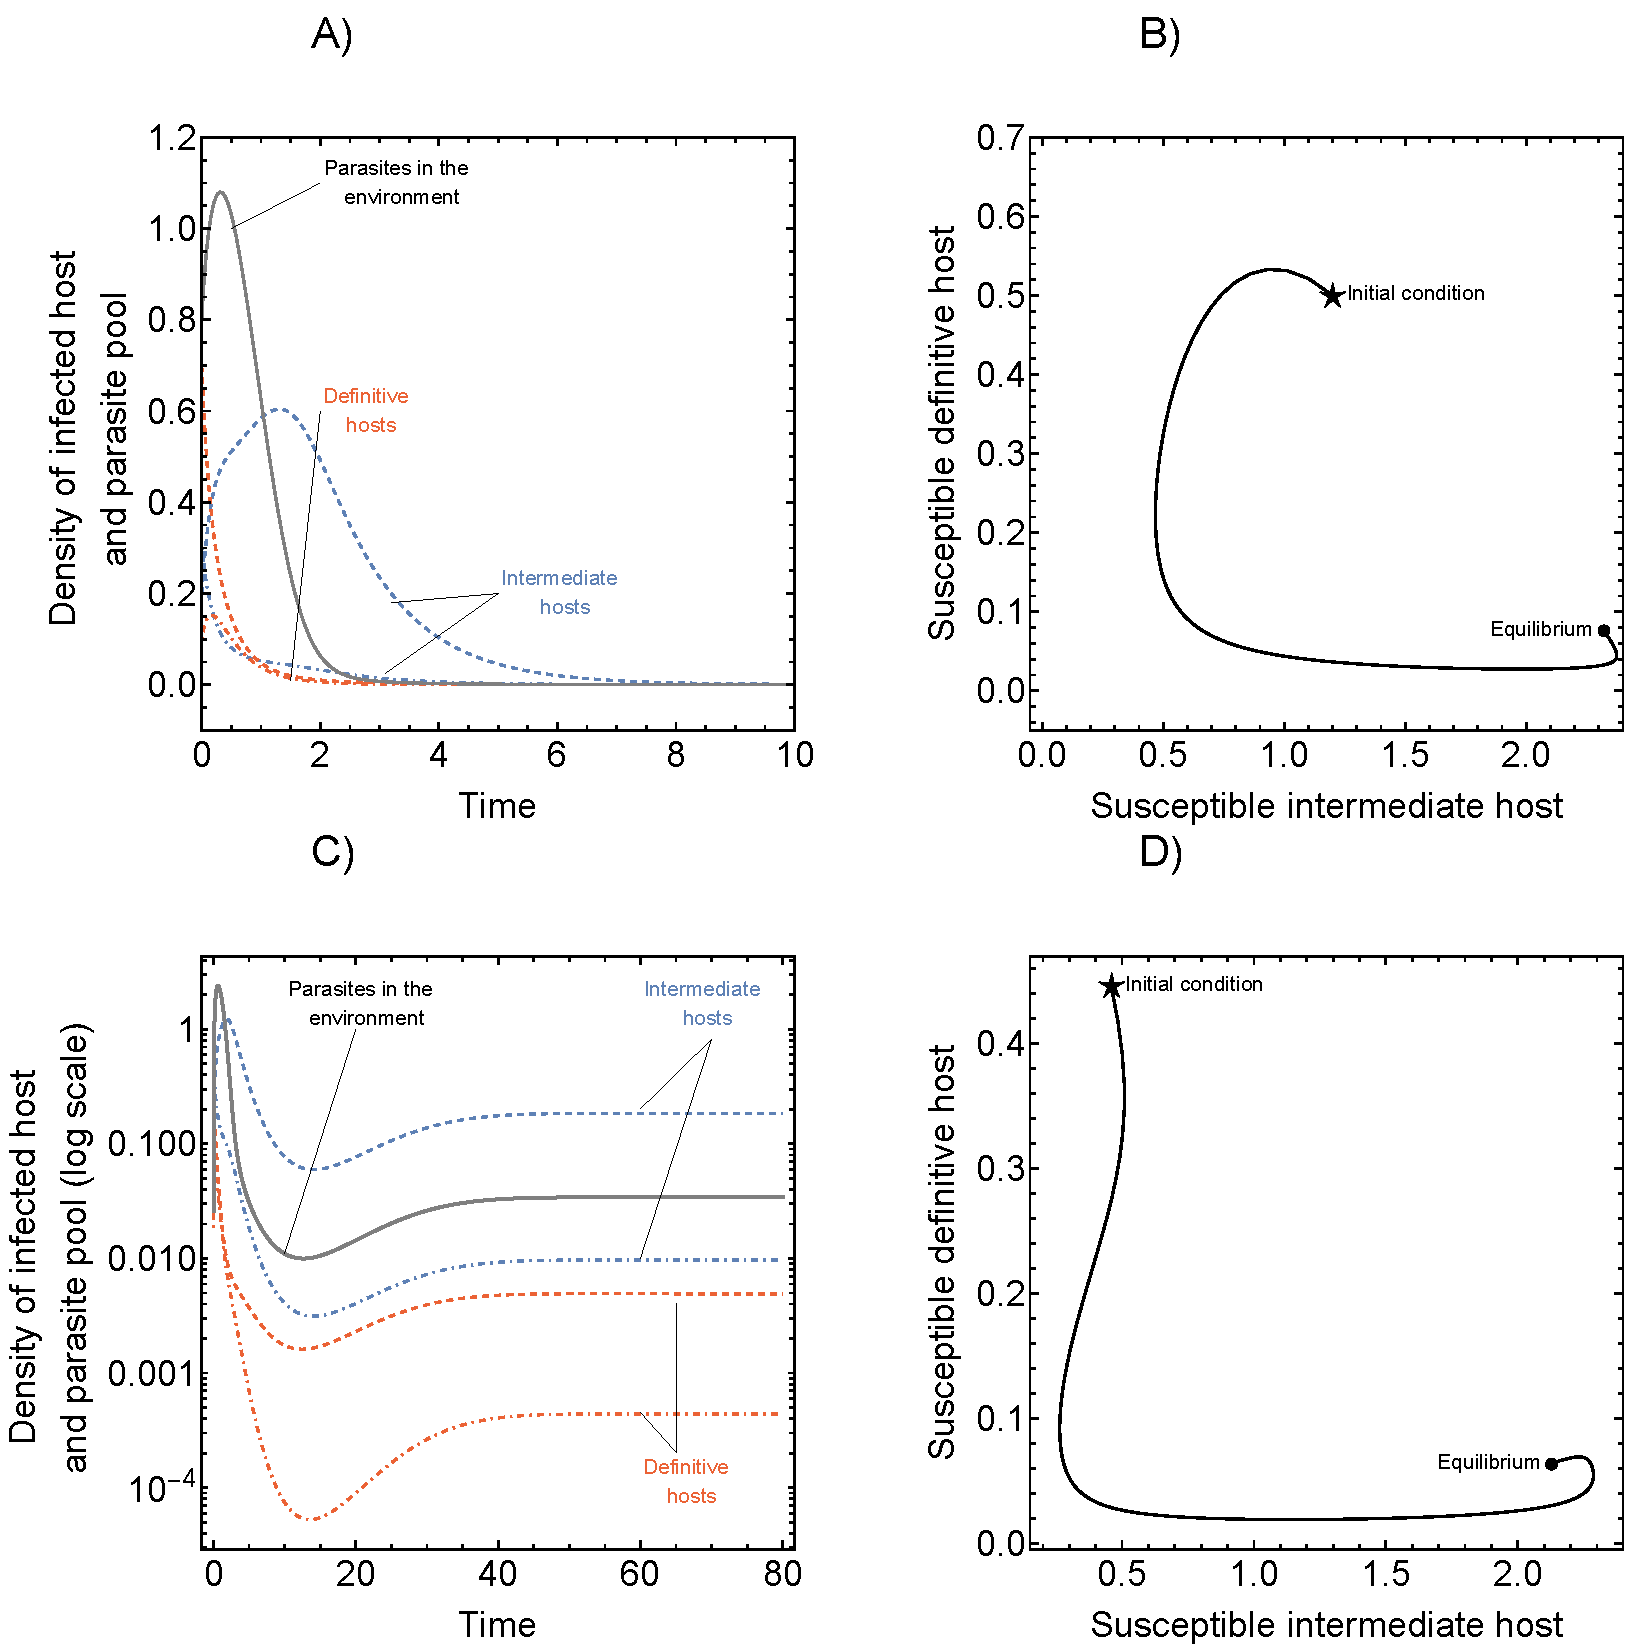
\includegraphics[width=\textwidth]{Figures/ecotraject_nonlinear.pdf}
\caption{A, B)Disease free equilibrium where parasite cannot persist. C, D) Disease stable equilibrium. Solid gray line indicate the density of free-living parasites, blue lines indicate infected intermediate hosts while red lines indicate infected definitive hosts. Dashed lines indicate singly infected hosts while dot-dashed lines indicate doubly infected hosts. Parameters for disease free equilibrium $\rho =  1.2, \ d = 0.9, \  r = 2.5, \ \gamma =  2.9, \alpha_w = \alpha_{ww} =  0, \ \beta_w = \beta_{ww} = 1.5, \ p = 0.05, \  c = 1.4, \ \mu = 3.9, \ \sigma_w = \sigma_{ww} = 0, \ q = 0.05, \ f_w = f_{ww} = 7.5, \ \delta = 0.9, \ k = 0.26, \ h_1 = h_2 = 0.6$. Disease stable equilibrium have the same parameter values except for higher host manipulation $ \beta_w =  \beta_{ww} = 4.5$ and parasite reproduction $ f_w  = f_{ww} = 45$}
\label{fig:ecotraject:nonlinear}
\end{figure}

When a parasite appears in the disease-free equilibrium, it spreads if its reproduction ratio $R_0 > 1$. 
Since the expression is complicated, we could not obtain analytical solutions for this inequality without assumptions. 
We assume the same parasite virulence, $\alpha_w = \alpha_{ww}$, $\sigma_w = \sigma_{ww}$, and reproduction in double infection as a linear function concerning reproduction in single infections, $f_{ww} = \epsilon f_w$. 
When $\epsilon > 1$, reproduction in double infections is enhanced as compared to in single infections, whereas $\epsilon \leq 1$, reproduction in double infections is depressed or equal to reproduction in single infections.
We found that the parasite can establish if its reproduction value in a single infection $f_w$ is more significant than a threshold (Figure \ref{fig:bistability}, see SI5). 

Our numerical results show that the parasite reproduction is substantial compared to other parameters (its value is nearly 40 times greater than other parameters).
This observation suggests that trophically transmitted parasites must release many offspring into the environment to persist. 
Interestingly, bistability occurs if the reproduction rate of the parasite in double infections is enhanced (Figure \ref{fig:bistability}A, B). 
In the bistable region, the parasite population can reach a stable equilibrium if the initial density is large enough. 
In contrast, with sufficient disturbance, the parasite population could go extinct.

\begin{figure}[!ht]
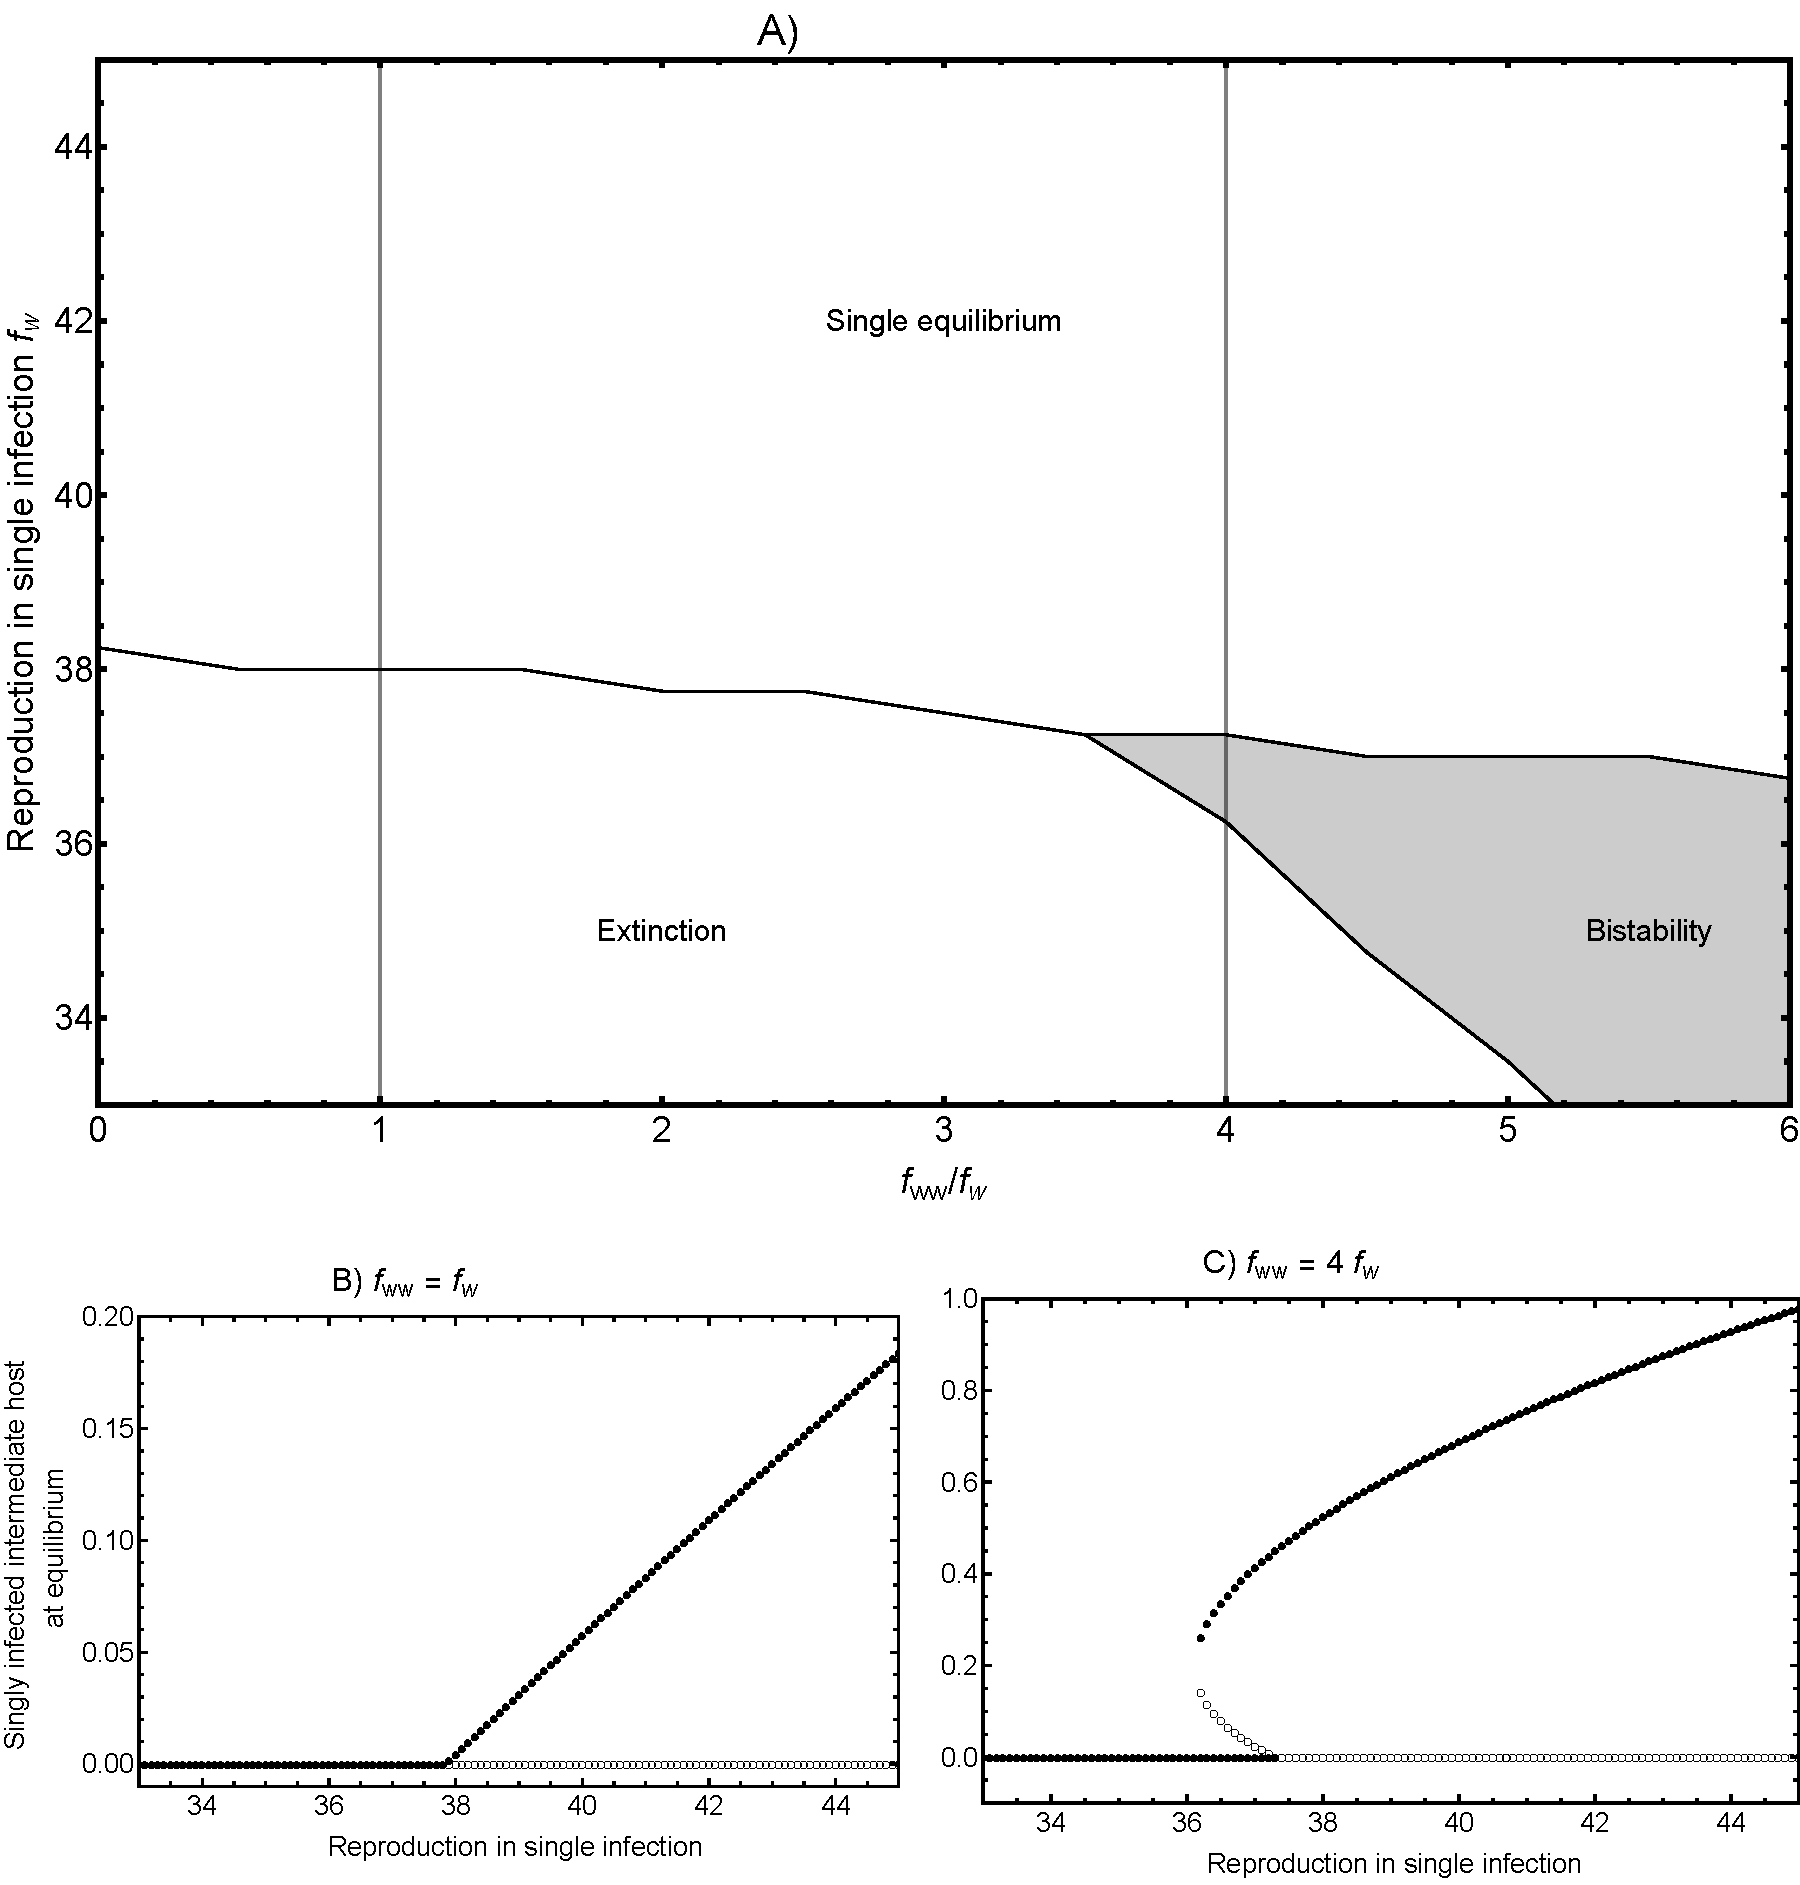
\includegraphics[width = \textwidth]{Figures/reproduction_bifurcation.pdf}
\caption{Effect of parasite reproduction on the ecological dynamics. A) Enhanced reproduction in double infection leads to bistability, B, C) Density of singly infected host at equilibrium when reproduction of parasites are the same in singly and doubly infected hosts $f_{ww} = f_w$, and when reproduction of parasites in doubly infected hosts is enhanced four times than those in singly infected hosts $f_{ww} = 4 f_w$. Filled circles indicate stable equilibrium and open circles indicate unstable equilibrium. Parameter $\rho = 1.2, \  d = 0.9, \  r = 2.5, \ \gamma = 2.9, \ \alpha_w = 0, \ \alpha_{ww} =  0, \ \beta_w = 1.5, \ \beta_{ww} = 1.5, \ p = 0.05, \  c = 1.4, \ \mu = 3.9,  \ \sigma_w = 0, \ \sigma_{ww} = 0, \  q = 0.05, \ \delta = 0.9, \ k = 0.26, \ h_1 = h_2 = 0.6$
}
\label{fig:bistability}
\end{figure}

\subsection*{The effect of host manipulation on ecological dynamics}

Host manipulation can be cooperative; two parasites increase the predation rate on intermediate hosts, or $\beta_{ww} > \beta_w$. 
However, it can also be uncooperative; the predation rate on doubly-infected intermediate hosts is lower than that on singly-infected ones or $\beta_{ww} < \beta_w$.
Cooperation in parasite manipulation increases the parasite's basic reproduction ratio $R_0$, but the manipulation in a single infection substantially affects the value of $R_0$ (Figure \ref{fig:manipR0}). 
Intuitively, if the manipulation in a single infection is minor, there is not enough transmission, and the parasite goes extinct.
However, suppose the ability to manipulate the host in a single infection is merely enough for the parasite population to escape extinction. 
In that case, cooperation in host manipulation leads to a bistable system state. 
Within the bistable region, the basic reproduction ratio can be less than one, suggesting that the parasite cannot spread when its manipulative values are within this area of weak manipulation when coinfected. 

\begin{figure}
\centering
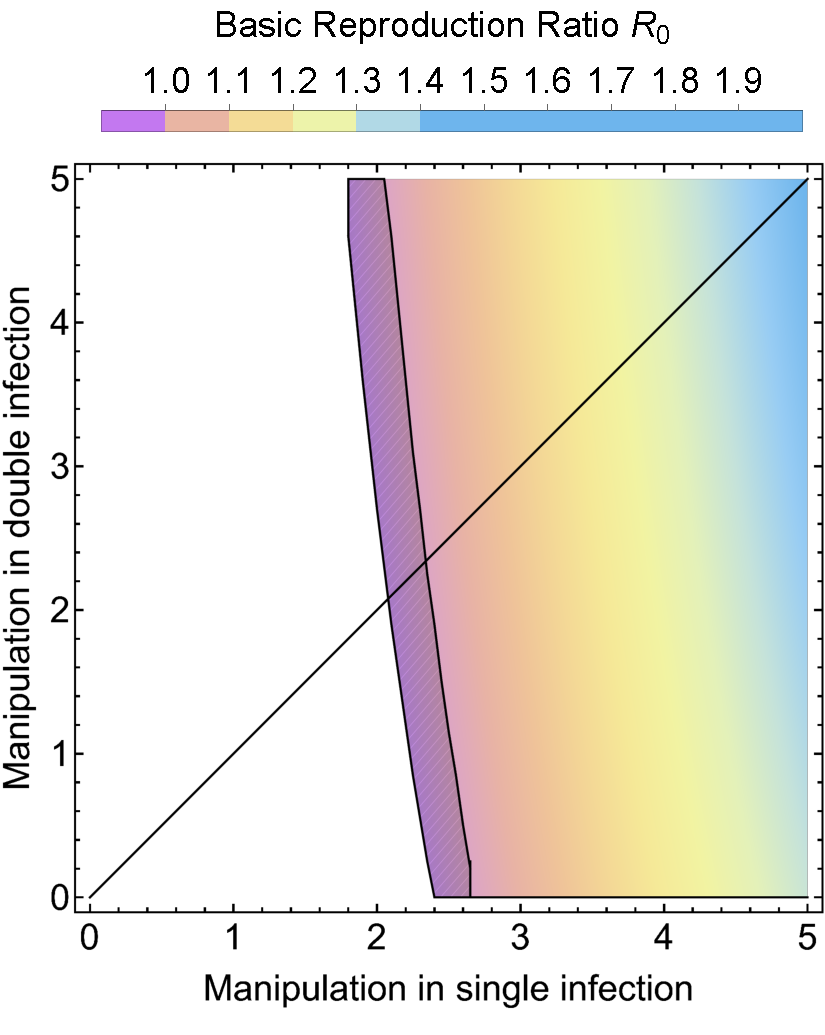
\includegraphics[width=0.5\textwidth]{Figures/manip_bifur_R0.pdf}
\caption{$R_0$ values increase with more efficient manipulation in both single and double infection. The parasite goes extinct if its manipulative ability is insufficient (white area). Bistability region occurs when cooperation in manipulation is intermediate (hatched area). As manipulation in single infection increases, the system only has one stable equilibrium. On the black line, manipulation is indifference between single infection and double infection ($\beta_w = \beta_{ww}$). Other parameters are the same as in Figure \ref{fig:bistability} and $f_w = 37 $}
\label{fig:manipR0}
\end{figure}

Co-infecting parasites can influence each other in different life history traits besides manipulation.
Parasites can have an enhanced reproduction rate in coinfections, i.e. $f_{ww} > f_w$. 
Likewise, they can compete for resources, so reproduction in double infection is depressed as compared to in single infection. 
Without any assumption on the relationship between manipulative ability and reproduction, we explore all possible combinations of cooperation-sabotage range in manipulation and depressed-enhanced range in reproduction.
If parasites are uncooperative in manipulations and shows depressed reproduction, they cannot persist (Figure \ref{fig:manipbifur}). 
In contrast, if they are highly cooperative in manipulation and show enhanced reproduction (i.e. $\beta_{ww}/\beta_w \rightarrow \infty$ and $f_{ww}/f_w \rightarrow \infty$), there is a guaranteed single equilibrium for parasite existence. 

For intermediate levels of coordination in reproduction and manipulation, a bistable area could occur.
However, the size of this area is sensitive to the value of reproduction and manipulation in a single infection. 
In particular, higher values of these two parameters reduce the bistability area, whereas larger values increase the bistability area (Figure \ref{fig:manipbifur}, Figure SI1).
If the parasites sabotage each other, the system is highly prone to bistability and only has a single equilibrium when reproduction is especially enhanced.
Interestingly, sufficiently high reproduction enhancement leads to bistability (i.e. $f_{ww}$ is at least four times $f_w$), and depressed reproduction always leads to a single equilibrium of the system (Figure \ref{fig:manipbifur}). 
While a single equilibrium guarantees the existence of a parasite population, bistability indicates that a disturbance of the system may likely lead to the extinction of the parasite population. 
This suggests that the benefits of coordination in reproduction and manipulation are context-dependent. 
Coordinating holds an advantage if there are no significant tradeoffs and if reproduction or manipulation in single infections are large enough. 

\begin{figure}[!ht]
\centering
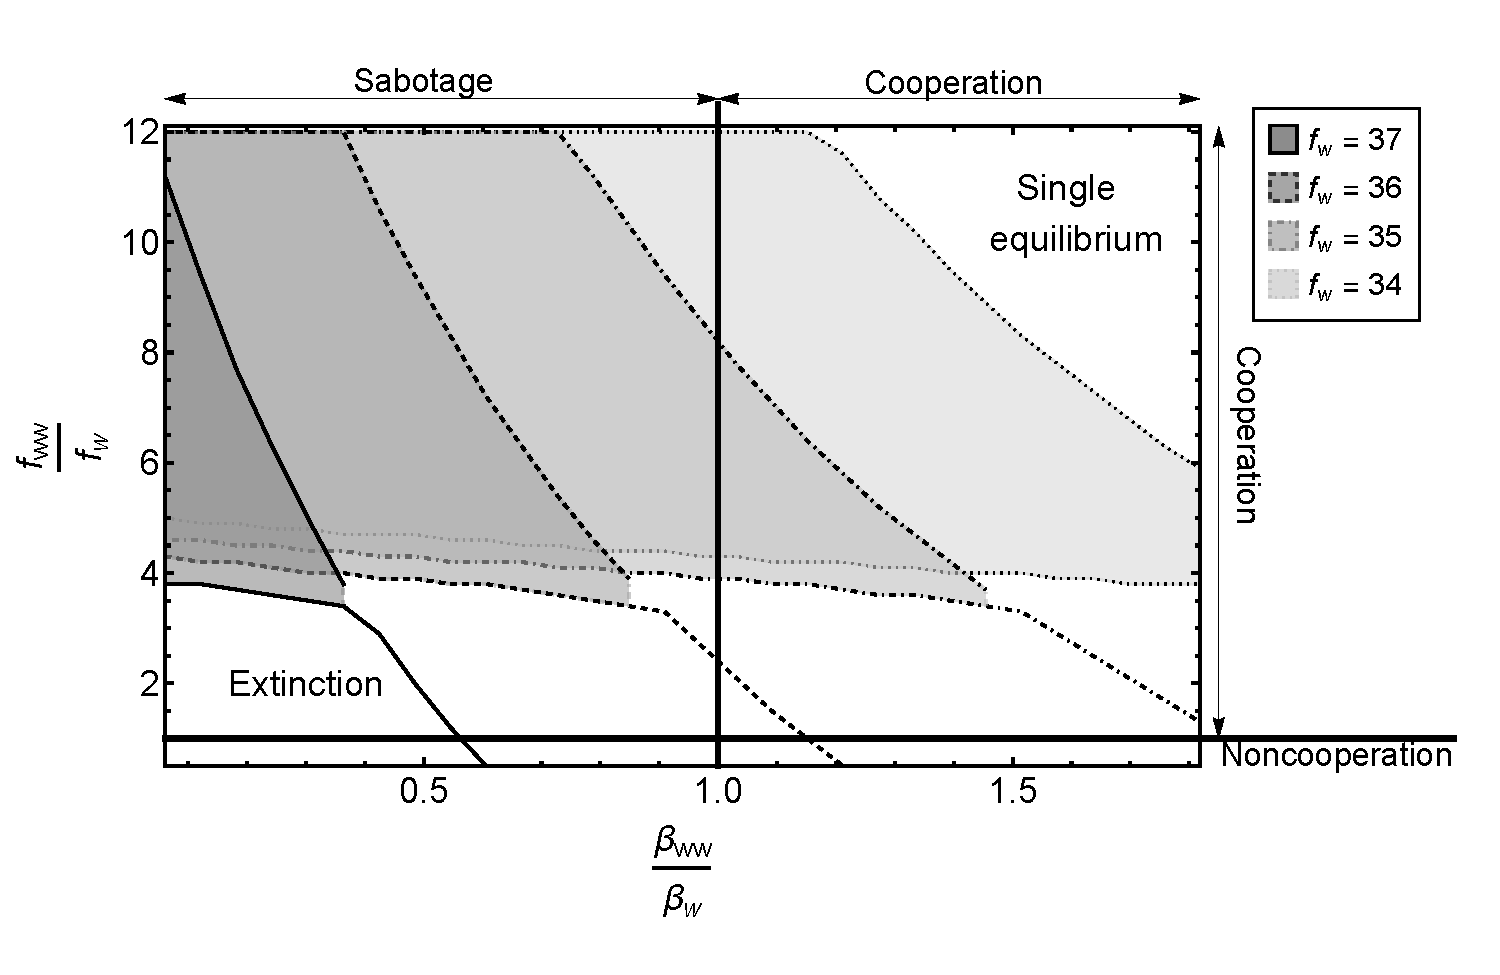
\includegraphics[width=\textwidth]{Figures/ratio_reproduction_manipulation.pdf}
\caption{Changes of the bistability area (shaded areas) with respect to different reproduction rates in single infection (different boundary styles). Manipulation and reproduction is indifference between single infection and double infection on the vertical and horizontal lines respectively. Common parameter:  $\rho = 1.2, \ d = 0.9, \ r = 2.5, \ \gamma = 2.9, \ \alpha_w = 0, \ \alpha_{ww} = 0, \ p = 0.05, \ c = 1.4, \ \mu = 3.9, \ \sigma_w = 0, \ \sigma_ww = 0, \ q = 0.05, \ \delta = 0.9, \ k = 0.26, \  \beta_w = 1.65, h_1 = h_2 = 0.6$.}
\label{fig:manipbifur}
\end{figure}

Co-transmission probability from the parasite pool to intermediate hosts $p$ has the opposite effect on the bistable area compared to co-transmission probability $q$ from intermediate hosts to intermediate hosts (Figure \ref{fig:contransmission}). 
In particular, when the parasite sabotages the manipulation, increasing $p$ enlarges the bistable area, whereas increasing $q$ reduces it. 
In contrast, when parasites cooperate in manipulation, reducing $p$ decreases the bistable area while reducing $q$ widens it.  
If cooperation in manipulation is exceptionally high, the population will always exist with one stable equilibrium regardless of the co-transmission value.
However, as there are always limitations and trade-offs, high values may not be possible.
Bistability indicates vulnerability to disturbance, suggesting that cooperation in manipulation may be beneficial when the co-transmission from the pool to the intermediate host increases. 
However, cooperation in manipulation may harm the population when the co-transmission from the intermediate host to the definitive host increases.

\begin{figure}[!ht]
	\centering
	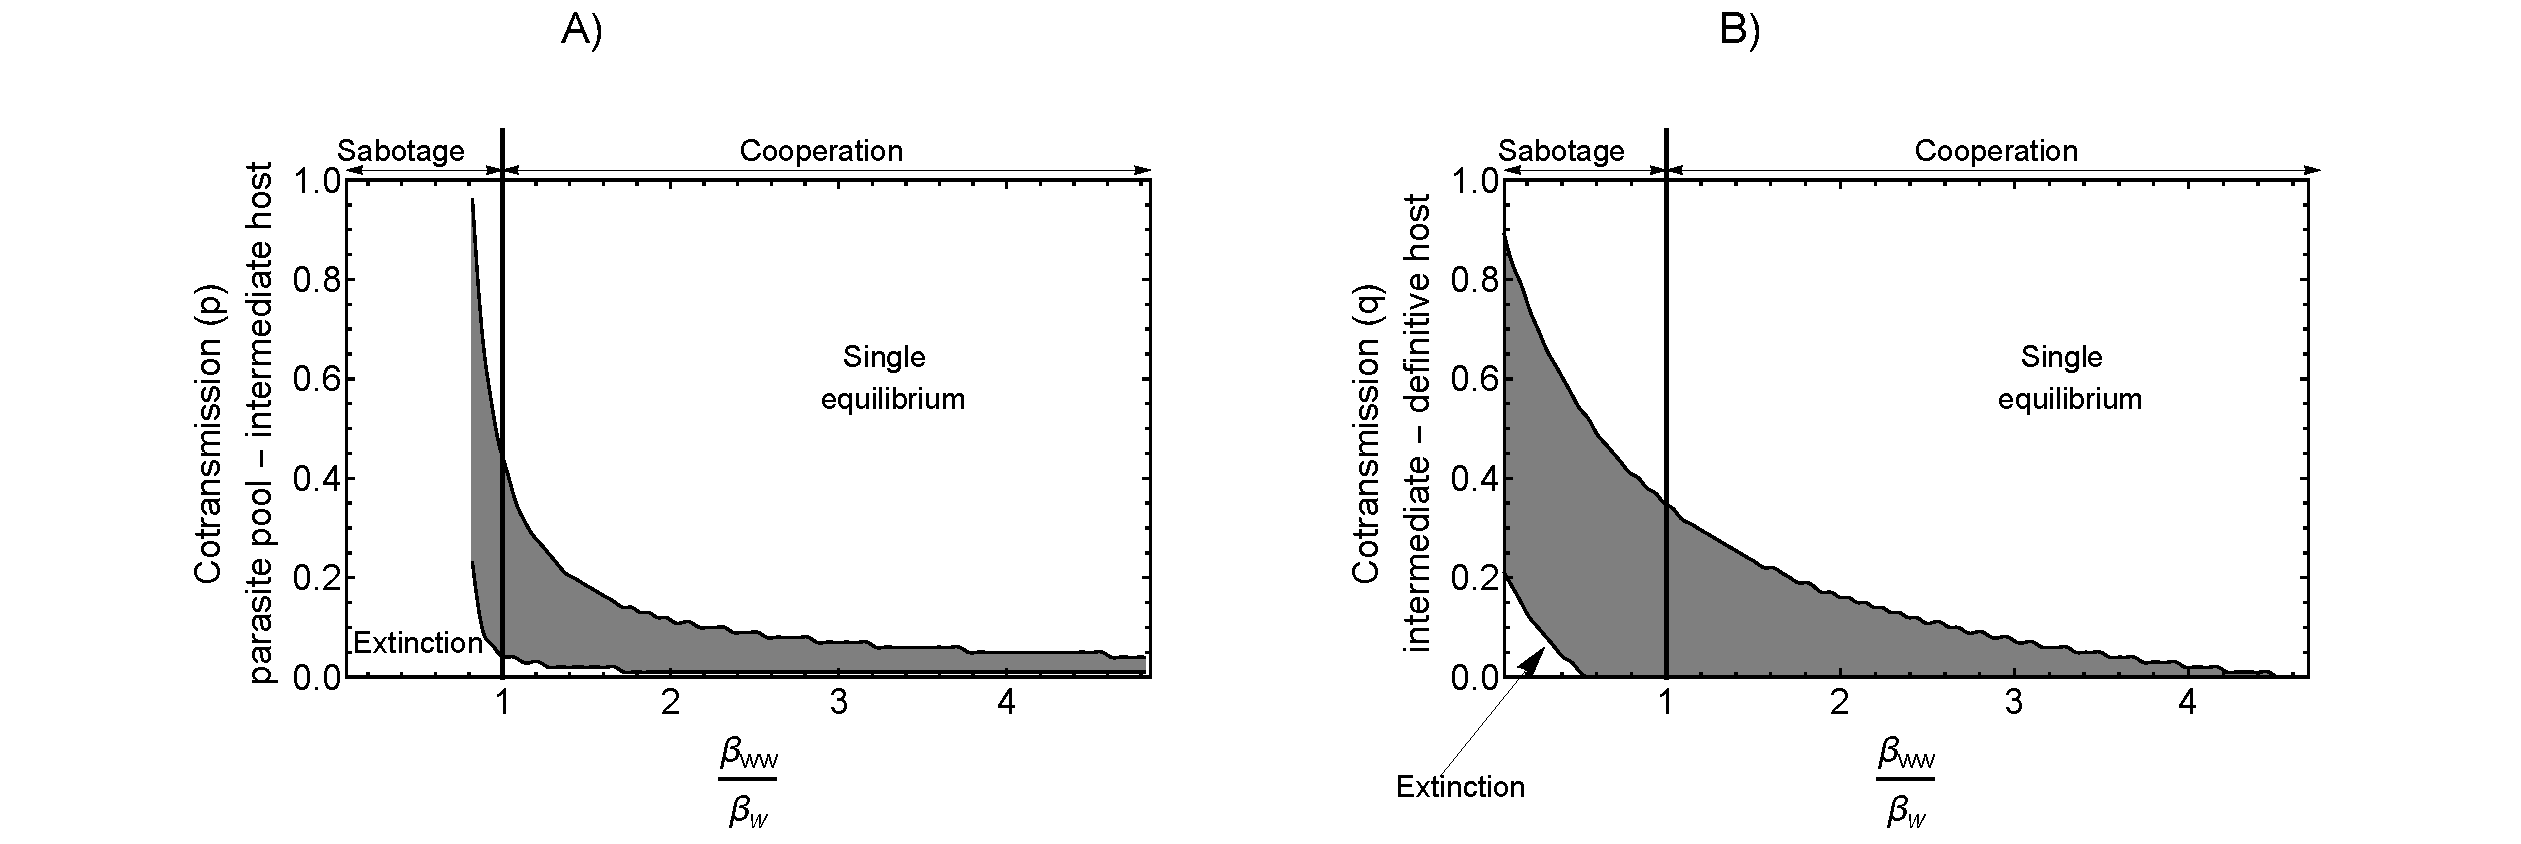
\includegraphics[width=\textwidth]{Figures/coinfect_transmission.pdf}
	\caption{\cha{Left: Effect of cotransmission from parasite pool to intermediate host. Right: Effect of cotransmission from intermediate to definitive host.} Common parameters:  $\rho = 1.2, \ d = 0.9, \ r = 2.5, \ \gamma = 2.9, \ \alpha_w = 0, \ \alpha_{ww} = 0, \ p = 0.05, \ c = 1.4, \ \mu = 3.9, \ \sigma_w = 0, \ \sigma_ww = 0, \ q = 0.05, \ \delta = 0.9, \ k = 0.26, \ \epsilon = 4.5, \ \beta_w = 1.45, \ f_w = 38, \ h_1 = h_2 = 0.6$.}
	\label{fig:contransmission}
\end{figure}

\section*{Discussion \& Conclusion}
Host manipulation is a ubiquitous phenomenon suggested to affect the prey-predator dynamics in trophically transmitted parasites. 
In particular, manipulation of infected intermediate hosts to increase the predation rate of definitive hosts may result in a heavy burden of predators on the intermediate host population.
This pressure can make parasites more vulnerable to extinction \citep{Hadeler1989,Fenton2006}. 

Our model shows that parasites cannot spread quickly in a cyclic predator-prey system. 
This delay is an expected result since even though the parasite's basic reproduction ratio $R_0$ is larger than one, it is estimated at the predator and prey's unstable equilibrium (or cyclic equilibrium). 
Thus, when the density of the prey and predator is at the minimum value of the cycle, the ''effective'' $R_0$ of the parasite can be smaller than one. 
Another interesting result is that the reproduction value is much larger than other parameter values.
This result is likely due to the introduction of a free-living parasitic pool. Our model shows that in making the system more realistic, we also obtain a more realistic quantitative value for parasitic reproduction.

In the study by \cite{Rogawa2018}, a non-manipulative parasite can invade a susceptible prey-predator population and cause the system to cycle. 
The system stops cycling and approaches a fixed point when the parasite becomes manipulative, and this stability increases with increased manipulation.
In our model, non-manipulative parasites cannot persist in the system, and the parasite never leads to cyclic dynamics. 
These results may contradict with \cite{Rogawa2018}, where non-manipulative parasites can still exists via cyclic behaviour. 
We suggest that the different results may be due to our introduction of a parasite pool and multiple infections, unlike the model of \cite{Rogawa2018}. 
In their system, transmission from the definitive host to the intermediate host was assumed to result from direct contact between the two hosts. 
Such immediate transmission could directly accelerate the feedback loop between prey and predator. 
Hence, faster predator-prey dynamics occur, which may lead to cyclic dynamics when parasites are introduced.

In our study, population dynamics exhibit bistability under certain circumstances. 
This is very likely due to the introduction of co-transmission, which has been shown to result in bistable population dynamics in plant virus \cite{allen_modelling_2019} and infectious diseases \cite{gao_coinfection_2016-1}.
 In this bistability region, if the system is disturbed (e.g. migration of the intermediate or definitive hosts or predation of intermediate hosts by other predators), then the density of the infected hosts may crash, leading to parasite extinction. 
The bistability region widens as parasites show enhanced reproduction but sabotage manipulation. 
This extension is because the density of the doubly infected hosts is always much smaller than the singly infected hosts, limited by sequential transmission and a small probability of co-transmission. 
If manipulation in a single infection is not sufficient then the transmission of the parasites depends mainly on the doubly infected hosts, which is rare. 
So, extinction is possible if manipulation in double infections is low.

\cite{Iritani2018} show that manipulative parasites persist if they can alternate manipulation between boosting and suppressing predation rate. 
In our model, the parasite cannot switch its manipulative strategy. 
Sabotaging manipulation reduces the basic reproduction ration $R_0$ and makes the system bistable, exposing the parasite to the risk of extinction. This result contrasts with \cite{Iritani2018} because in our model, sabotage decreases transmissmion rate from intermediate to definitive host, and does not benefit the parasite.

Finally, our study focuses on the ecological dynamics of the trophically transmitted parasite. 
However, investigating the evolution of host manipulation is a natural extension beyond the scope of a single manuscript, given the complexities that arise in the ecological dynamics itself.
Studying the evolution of host manipulation, considering the free-living parasite pool, calls for thorough analyses, which could be a standalone study. 
For example, we would need to include differences between the traits of the multiple parasites and hence the ecological model becomes more complex than presented in this study.
The combinatorics and orderings of sequential infections wil lthen become important.
In addition, the occurrence of bistability in our model suggests that the evolution of host manipulation may drive the parasite to extinction simply because of the rarity of the mutant and the Allee effect as per Adaptive dynamics approaches. 
The coinfecting parasites can increase manipulation and enhance reproduction freely if there exist no tradeoffs. 
Nevertheless, our model shows that the benefits of this strategy are context-dependent, making it suboptimal in certain cases. 
Evolutionary dynamics would therefore depend on the tradeoff between host manipulation and other traits of the parasites, such as reproduction, virulence, and survivorship in the parasite pool, to list a few. 
This extension deserves thorough analysis, and we will treat it as a separate matter.


\section*{Acknowledgements} 
We thank the Swiss National Science Foundation Sinergia grant no CRSII5\_202290 for supporting Phuong Nguyen to work on this manuscript as a side project.
Funding from Bayerische Forschungsallianz and from the Max Planck Society if gratefully acknowledged (CSG).
We also thank Tina Scheibe for helpful discussions.
This paper is dedicated to the memory of Martin Kalbe, an exceptional parasitologist who made remarkable contributions to the field.
Beyond his academic prowess, Martin was a truly exemplary friend and human being, touching the lives of those around him with his warmth, kindness, and unwavering support.

\section*{Statement of Authorship}
Both authors developed the theory.
P.L.N developed and implemented the computational model.
Both authors wrote the manuscript.
 
\section*{Data and Code Availability}
All data and simulation codes for generating figures are available on 
\url{https://anonymous.4open.science/r/multipleinfections}

\bibliographystyle{evolution}
\bibliography{references}

\section*{Tables}
\renewcommand{\thetable}{\arabic{table}}
\setcounter{table}{0}

\begin{table}[!ht]
\caption{Description of variables and parameters}
\label{table:varpardescription}
\centering
\begin{tabular}{c|p{10cm}}%{|p{2.5cm}|p{12cm}|} 
\hline
Parameters and Variables    &  Description  \\
\hline
$I_i$  & Density of intermediate hosts that are susceptible $i=s$, singly infected $i=w$, or doubly infected $i=ww$ \\
\hline
$D_i$ & Density of definitive hosts that are susceptible $i=s$, singly infected $i=w$, or doubly infected $i=ww$ \\
\hline
$W$ & Density of parasites released from definitive hosts into the environment \\
\hline
$d$ & Natural death rate of intermediate hosts \\
\hline
$\alpha_i$ & Additional death rate of intermediate hosts due to infection by a single parasite ($i = w$) or two parasites ($i = ww$) \\
\hline
$p$ & Probability that two parasites cotransmit from the environment to an intermediate host \\
\hline
$\gamma$ & Transmission rate of parasites in the environment to intermediate hosts \\
\hline
$\mu$ & Natural death rate of definitive hosts \\
\hline
$\sigma_i$ & Additional death rate of definitive hosts due to infection by a single parasite ($i = w$) or two parasites ($i = ww$) \\
\hline
$\sigma_i$ & Additional death rate of the hosts due to being infected by a singly parasite ($i = w$) or two parasites ($i = ww$) \\
\hline
$q$ & Probability that two parasites cotransmit from intermediate hosts to definitive hosts \\
\hline
$\beta_i$ & Transmission rate of parasites from intermediate hosts to definitive hosts \\
\hline
$f_i$ & Reproduction rate of parasites in singly infected definitive hosts ($i = w$) or doubly infected hosts ($i = ww$)\\
\hline
$\delta$ & Natural death rate of parasites in the environment \\
\hline 
$h$ & Probability that the parasites successfully established inside the definitive host 
\end{tabular}
\bigskip{}\\
\end{table}

\end{document}